\chapter{Krav}\label{ch:krav}


Nu hvor der er lavet en god business model og case, vil kravene nu præciseres ud fra den systemvision der er lavet, og de use cases der er stillet op. Dette indgår i Elaboration fasen, som indeholder en bladning af at planlægge og modellere projektet. Dette betyder at de tidligere Use Cases implementeres, og det vil vise hvordan softwarens arkitektur beskrives og hvilke forudstæninger der bliver sat. I Inception fasen var der et større fokus på at forstå scopet og en lille del af kravende, i tekst form. Men i Elaboration fasen vil de fleste uml diagrammer finde sted\cite{Larman2004}. Herunder befinder Krav, Analyse, Desing og Test aktiviterene sig under Elaboration fasen i Unified Process\cite{UnifiedProcess}. 

\section{Funktionelle krav}\label{sec:funktionelle-krav}
Dette afsnit vil behandle de funktionelle krav der skal være til systemet. De funktionelle krav omhandler de krav, der stilles til funktionaliteten af programmet gennem use cases\cite{Larman2004}. 

\subsection{Fully Dressed} \label{fullydressed}
Herunder ses Fully Dressed Use Casen Automatisk lagerstyring. Use case Automatisk Lagerstyring er bygget på de tidligere use cases: Afskriv vare, fordi den påvirker hvor meget der er på lager. Optælling af isbil, som er manuelt arbejde og vil nemt kunne erstattes med automatisk optælling. Bestil varer, ville gå hånd i hånd med automatisk optælling af bilen. Og til sidst use case Modtag varer, fordi systemet skal opdateres med de nye varer der kommer på lager. 

De alternative flows beskrevet i diagrammet er fundet gennem en diskussion, hvor mulige fejl eller forhindringer kan opstå under flowet af handlinger. De alternative flows beskriver, hvordan et system kan fejle undervejs, hvad der er nødvendigt at være forberedt på, og hvordan disse alternative flows kan behandles så systemet ikke stopper, men kan fortsætte Use Casen til ende. Sker det at systemet eller kunden ikke opfører sig som forventet, skal de mulige udfald udtænkes, og sådanne scenarier skal kunne behandles af systemet så vidt muligt.

\todo{update so it's consistent with new ssd}
\begin{longtable}{ |p{120pt}|p{120pt}|p{120pt}| }
    \hline
    \textbf{Use case navn} & Automatisk lagerstyring & \\
    \hline
    \textbf{Aktør} & Depotchefen & \\
    \hline
    \textbf{Præbetingelser} & Et lager med en addresse, penge til at bestille, lager og isbiler er talt op og salgsdata & \\
    \hline
    \textbf{Postbetingelser} & Et lager tilpas fyldt med is & \\
    \hline
    \textbf{Frekvens} & 1 gang om dagen & \\
    \hline
    \textbf{Main Success Scenario} (Flow of events) & \textbf{Aktørhandling} & \textbf{Systemsvar} \\
    \hline
    & 1. Aktøren trykker på "Lager" & 2. Viser lagerbeholdning \\
    \hline
    & 3. Klikker på "Generer lagerplan" &  \\
    & & 4. Planen gemmes og sendes automatisk til plan-fanen \\
    \hline
    & 5. Klikker "Åben plan" & 6. Viser bestillingsplanen med mulighed for at kunne rette i den estimerede bestillingsplan. \\
    \hline
    & 7. Gemmer rettelser ved at klikke "Gem plan" & 8. Opretter bestillinger af varer ud fra bestillingsplanen. \\
    \hline
    \textbf{Alternative flows} & 0.1 Udgåede eller ødelagte varer skal afskrives & \\
    \hline
    & 0.2 Afskrevne varer registreres i systemet. & 0.3 Lager status opdateret. \\
    \hline
    & 4.1 Aktøren vil gerne modificere planen, retter det i plan-fanen og gemmer planen & \\
    \hline
    & & 8.1 Planen er tom. Der kan ikke oprettes en bestilling. Giver en fejlbesked. \\
    \hline
\end{longtable}

\subsection{Kandidattabel}
Nu hvor den centrale Use Case er valgt, kan der nu laves Kandidatklasser. 
Ved opgaven Automatisk lagerstyring skal \textbf{brugeren} kunne se lagerbeholdningen i \textbf{fryseren}. Ud fra \textbf{salgsstatistik} og tilbud kan den optimale mængde \textbf{varer} bestilles hjem. Det skal være muligt at generere en \textbf{lagerplan}, åbne den, og oprette en eller flere \textbf{bestilling} med den.

\begin{longtable}{ |p{120pt}|p{120pt}|p{120pt}| }\label{fig:Kandidatklasser}
    %\hline %why the fuck doesn't this work?
    \textbf{Kandidat Til Klasse} & \textbf{Vurdering} & \textbf{Konklusion} \\
    \hline
    Fryser & Er en fysisk ting der køler is & OUT \\
    \hline
    Sale & Indeholder salgsoplysninger fra et salg ude ved kunden & klasse \\
    \hline
    Product & Indeholder productoplysninger - pris, ID & klasse \\
    \hline
    Customer & Indeholder kundeoplysninger & klasse \\
    \hline
    CustomerOrder & En ordre lavet af en kunde som skal leveres til kunden & klasse \\
    \hline
    DepotOrder & En bestilling af is til depotet & klasse \\
    \hline
    Seller & Indeholder sælgeroplysninger, bliver forbundet med Sale & sale \\
    \hline
    Boss & Indeholder adminstratoroplysninger & klasse \\
    \hline
    DepotPlan & Beskriver hvordan depotet skal ændre sig som sæsonerne gør & klasse \\
    \hline
\end{longtable}
Nu er Kandidatklasserne fundet, og det er nu muligt at opstille en domænemodel af systemet, så basisformen af systemet kan designes, samt forholdene mellem klasserne.


\section{Informationskrav}\label{sec:informations-krav}
\todo{introduktion og Unified process}

\subsection{Domænemodel}

\subsection{Domænemodel}\label{Domainmodel}
Domænemodellen beskriver de relationer klasserne har til hinanden, samt hvilke attributter de indeholder. Her laves domænemodellen ud fra Kandidatklasserne og arkitektur principper.

\begin{figure}[H]
    \centering
    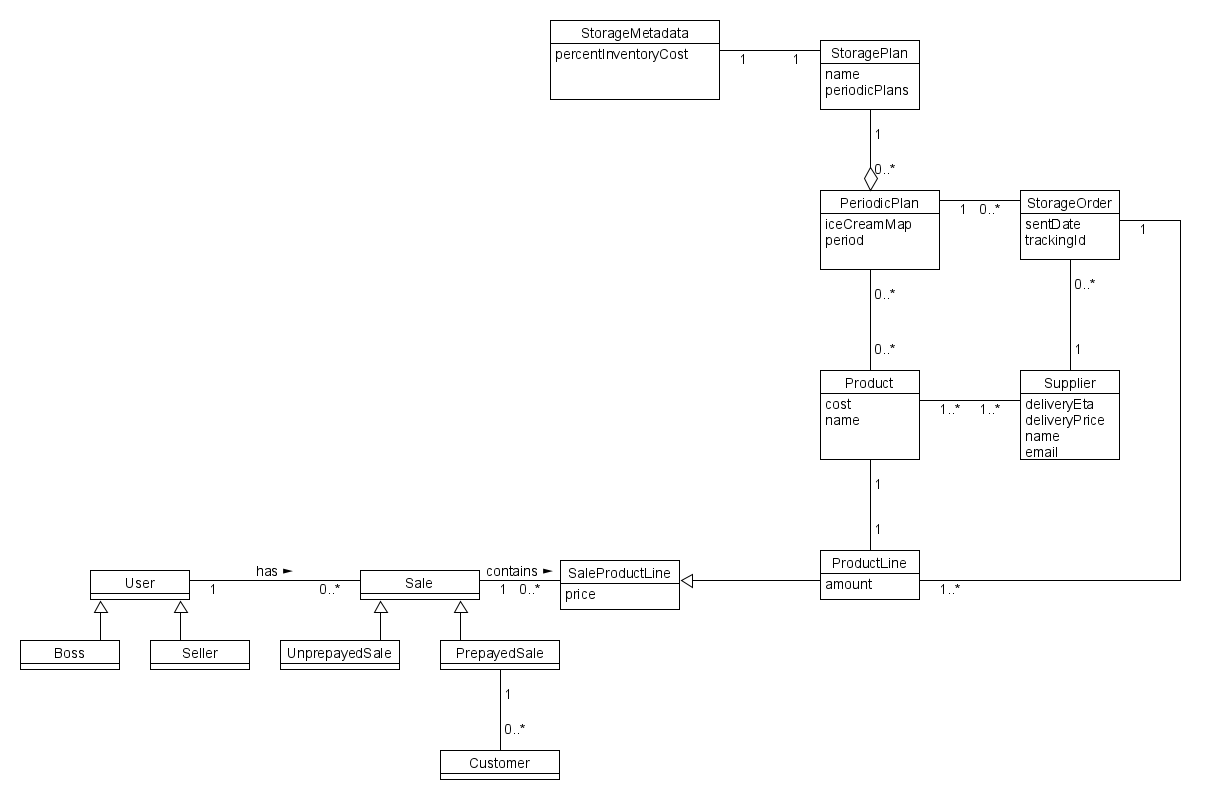
\includegraphics[width=0.9\textwidth]{figures/krav/domain_model_1.png}
    \caption{Domænemodel 1}
    \label{fig:domain_model}
\end{figure}

Domænemodellen som ses ovenfor viser hvordan klasserne er repræsenteret og hvilke relationer de har til hinanden. SeasonalPlan er planen, som beskriver hvordan lageret skal være hos Hjem-IS. Sæsonplanen for lagerbeholdningen bestemmes af hvilke produkter der er på lager, og hvor meget der bliver solgt. Ud fra dette kan der laves en bestilling (StorageOrder), som indeholder informationer om hvilke produkter der skal bestilles, hvilken Supplier de skal bestilles fra. Disse bestillingsplaner bestemmer sæsonplanen.
For at kunne gennemføre Use Casen er det ikke nødvendigt endnu at tage højde for Sales og Users, da det kun er Products og Storage ændringer der er relevante. 

\begin{figure}[H]
    \centering
    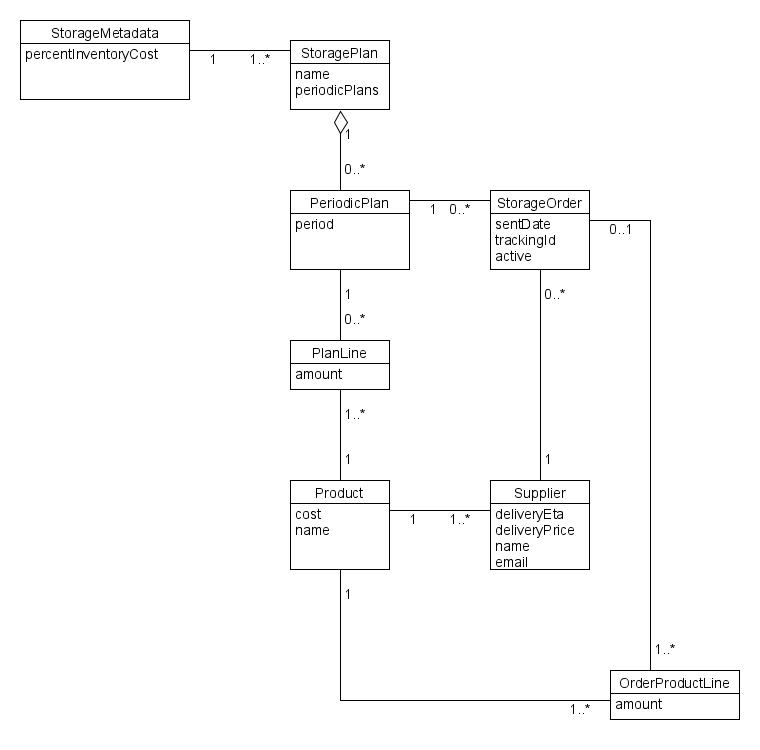
\includegraphics[width=0.9\textwidth]{figures/krav/domain_model_2.png}
    \caption{Domænemodel 2}
    \label{fig:domain_model_2}
\end{figure}

Domænemodellen ovenfor forholder sig kun til de relevante klasser for at kunne gennemføre Use Casen Automatisk Lagerstyring. Det er ud fra denne at databasen vil blive designet.

\subsection{Database}
\todo{normalisering}
Nu hvor domænemodellen er på plads kan der nu også udvikles en relational model af databasen. Der vil først tages udgangspunkt i at mappe hver klasse til en tabel, hvor der tages højde for klassenavn og attributter.
Da der ingen nedarvning er mellem nogen af klasserne, er det ikke relevant at tænke i pull-up og pull-down. Hver klasse får derfor sin egen tabel.
Dernæst skal associationerne laves ud fra om der er tale om 1-til-1, 1-til-mange eller mange-til-mange relationer. 

\begin{figure}[H]
    \centering
    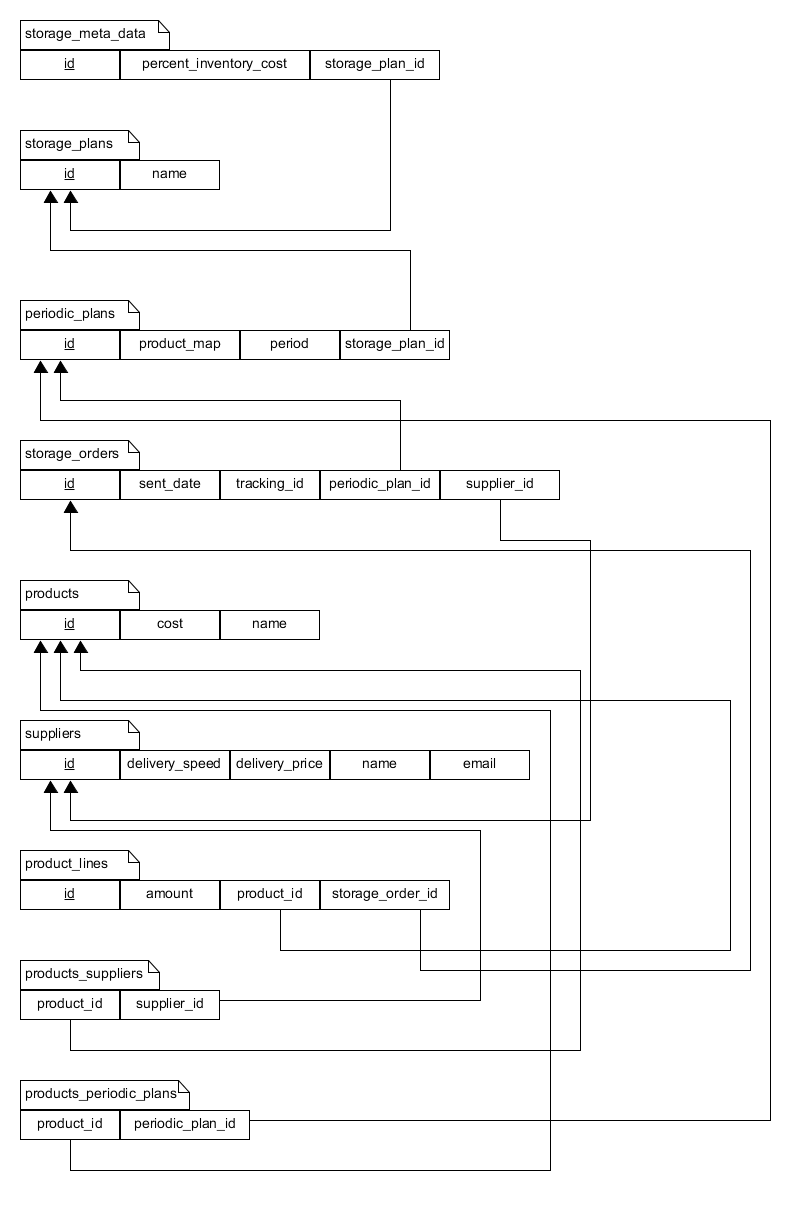
\includegraphics[width=0.9\textwidth]{figures/krav/relation_model_0th_normalization.png}
    \caption{Relationsmodel før normalisering}
    \label{fig:relational_model_0}
\end{figure}

Reglerne for de forskellige relationer og hvordan de skal forbindes er fulgt under udviklingen af den relationelle model, hvilket bl.a. kan ses på 'product_supplier' tabellen. Denne forbinder en mange-til-mange association mellem Product og Supplier. 
Nu hvor tabellen er lavet, kan den nu normaliseres.
Efter at have kigget tabellen igennem kan det ses at 1NF allerede er opfyldt, da samtlige værdier er atomiske.
For at opfylde 2NF skal 1NF være opfyldt, og der skal ikke være nogle partial dependencies. Efter endnu en vurdering er der ingen værdier som afhænger af en anden, hvilket betyder at relationalmodellen allerede opfylder 2NF.
For at opfylde 3NF skal 2NF være opfyldt, samt må der ikke være nogle transitive afhængigheder. Det minder meget om kravet til 2NF, og det kan igen konkluderes at der ingen transitive afhængigheder er.
For at opfylde BCNF kræves det at 3NF er opfyldt og at samtlige attributter er kandidatnøgler.


 